\section{Discussion and Comparison}

To discuss the effect and impact of adaptive and generative music on the player, three studies are first presented. The studies evaluate the subjective responses of the participants and compare these responses for environments with linear, adaptive or generative music.

\subsection{Study 1}
Hutchings and McCormack have adapted an AMS (adaptive music system) to the two video games "Zelda: Mystery of solarus" \cite{zeldamysteryofsolarus2011}  and "Starcraft ii: Wings of liberty" \cite{starcraftiiwingsofliberty} \cite{hutMcCormAms}. The system was integrated into the games so that it receives information about the current state of the game at runtime \cite{hutMcCormAms}. In addition, the musical output of the system was replaced with the output of the AMS \cite{hutMcCormAms}. 

The system was then evaluated in a study with 34 participants \cite{hutMcCormAms}. The participants were asked to provide information on their feeling of immersion, the quality of the music and the correlation between music and actions \cite{hutMcCormAms}. They were divided into two groups \cite{hutMcCormAms}. Group A plays the game "Zelda: Mystery of solarus" with original music and "Starcraft ii: Wings of liberty" with music from the AMS \cite{hutMcCormAms}. Group B runs through both games in the other environment \cite{hutMcCormAms}. This prevents a participant from playing one game in two different music environments and therefore reduces bias \cite{hutMcCormAms}.

Furthermore, during the evaluation, the participants were played a short section of music that represents a certain game state or is played at a certain point in the game \cite{hutMcCormAms}. The participants then had to assign a term for a concept from the game to this section of music that they thought best suit \cite{hutMcCormAms}. The four game concepts for the music sections are shown in Fig. \ref{fig:tutorial_gal_def}. Additional the accepted terms for every concept are listed. 
\begin{figure}
    \centering
    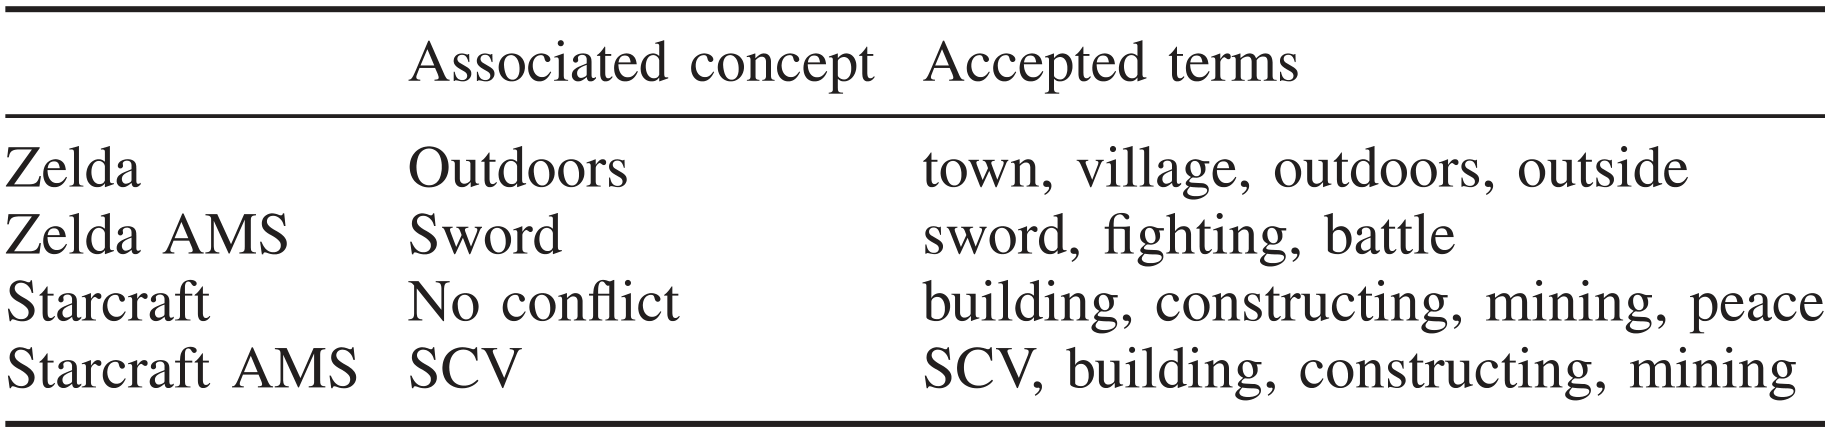
\includegraphics[width=1\linewidth]{images/ams_evaluation_table2.png}
    \caption{Accepted terms for established concepts \cite{hutMcCormAms}}
    \label{fig:ams_evaluation_table2}
\end{figure}
Participants of group A was played the music sections of the AMS conditions “Zelda AMS” and “Starcraft AMS” (see Fig. \ref{fig:tutorial_gal_def}) \cite{hutMcCormAms}. Group B was played the original music conditions “Zelda” and “Starcraft”) (see Fig. \ref{fig:tutorial_gal_def}) \cite{hutMcCormAms}.
For the “Zelda” condition, 70\% of participants stated a correct term. For the “Zelda AMS” condition, only 53\% of the participants reported one of the terms defined as correct \cite{hutMcCormAms}.
For music from the game “Starcraft ii: Wings of liberty” the results were similar with 59\% of participants assigning a correct term to the original music and 41\% of participants assigning a correct term to the music section of the AMS \cite{hutMcCormAms}.
This indicates that music from the AMS is more often misinterpreted and the associated game context is more likely to be confused than with the original, composed music.
However, the other reported results of the participants show a significant increase in the immersion and correlation of music and gameplay with the music output of the AMS compared to the original music \cite{hutMcCormAms}.

Hutchings and McCormack conclude that the AMS could be successfully applied to the games in this study \cite{hutMcCormAms}. Furthermore, they see the spreading activation model used for the AMS as a suitable model for analysing player emotions and game events \cite{hutMcCormAms}.

\subsection{Study 2}
Another study on the effects of adaptive music on the player was conducted by Plut and Pasquier \cite{plut2019music}. They created a video game called "Galactic Escape" using "FMOD Studio" \cite{fmod} to adapt the music to the gameplay \cite{plut2019music}. 25 participants took part in this study \cite{plut2019music}. Each participant played the game “Galactic defense” once with each of the four different music conditions (see Fig. \ref{fig:music_matters_table3}). The order of the music conditions was decided at random \cite{plut2019music}.
\begin{figure}
    \centering
    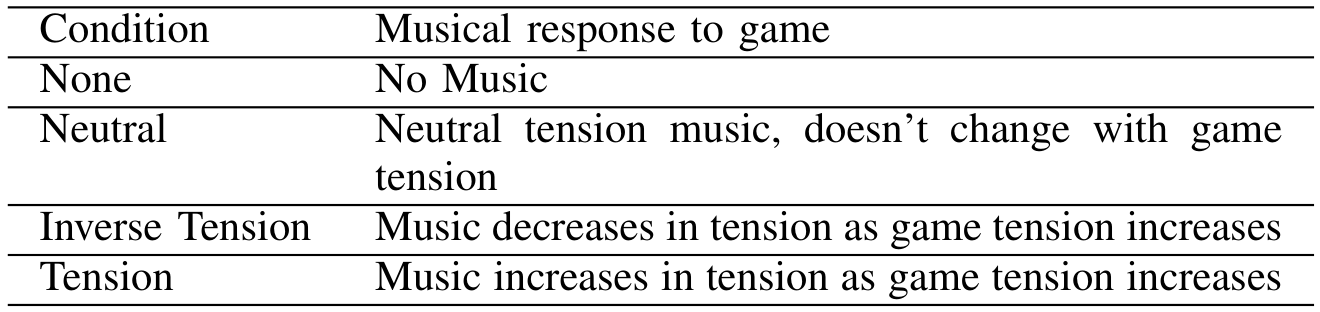
\includegraphics[width=1\linewidth]{images/music_matters_table3.png}
    \caption{Experimental conditions \cite{plut2019music}}
    \label{fig:music_matters_table3}
\end{figure}
After each game run, the participants report their enjoyment, affect and emotion by filling out a questionnaire \cite{plut2019music}. 

According to the results of the questions about enjoyment, the participants enjoyed the condition “None” (see Fig. \ref{fig:music_matters_table3}) without music the least \cite{plut2019music}. For the other three conditions the participants reported similar response values \cite{plut2019music}.

A greater difference between the conditions was reported for the perceived emotion \cite{plut2019music}. The participants indicate a higher response value for emotion in the "neutral" and "inverse tension" condition (see Fig. \ref{fig:music_matters_table3}) compared to the condition without music \cite{plut2019music}. For the "tension" condition, which features a congruent adaptation of music to the level of tension, the emotional response value is even higher than for the other conditions \cite{plut2019music}.

For the evaluation of the player's affect, Plut and Pasquier used a three-dimensional affect model with the dimensions valence, tension and arousal, which is a simplified version based on a more complex model by Schimmack and Grob \cite{schimmack2000dimensional} \cite{plut2019music}.
The questions about the player's affect are divided in one question for each dimension \cite{plut2019music}.
The response value for the dimensions arousal and valence show a similar trend and are similar to the emotional response (see Fig. \ref{fig:music_matters_experienced_affect}) \cite{plut2019music}. The arousal and valence value is higher for the "neutral" and "inverse tension" condition compared to the "none" condition without music \cite{plut2019music}. The values increase even further for the "tension" condition \cite{plut2019music}.
In contrast to this, the self-reported tension is decreased when music is introduced in the "neutral" condition compared to the "none" condition without music. However, it increases in the "inverse tension" and "tension" conditions, which feature adaptive music \cite{plut2019music}.
\begin{figure}
    \centering
    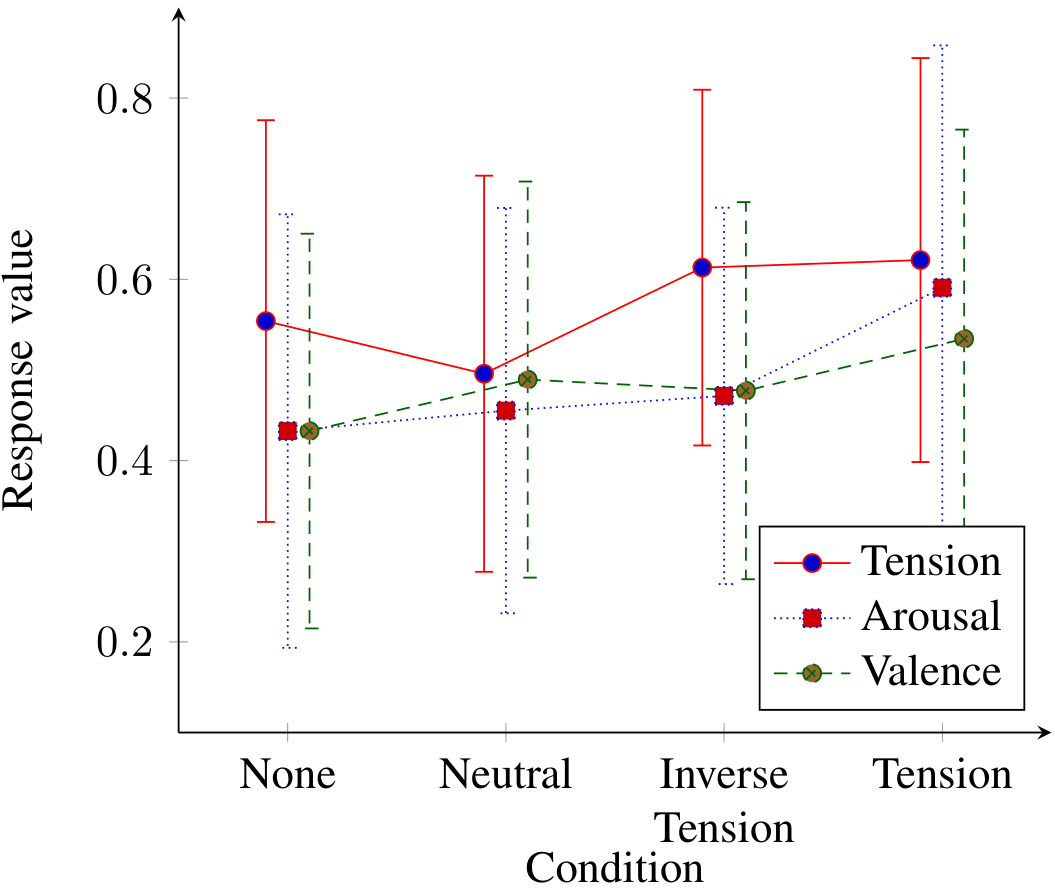
\includegraphics[width=1\linewidth]{images/music_matters_experienced_affect.png}
    \caption{Experienced affect means and Standard Deviations \cite{plut2019music}}
    \label{fig:music_matters_experienced_affect}
\end{figure}

The difference in self-reported tension between the "inverse tension" and "tension" conditions is minimal \cite{plut2019music}. This indicates that whether the music's tension adaptively matches the game's tension ("tension" condition) or is inversely adaptive to the game's tension ("inverse tension" condition), participants reported similar tension levels \cite{plut2019music}. Plut and Pasquier conclude from this that the adaptivity of the music is generally more important than the congruence between the game's tension and the music's tension \cite{plut2019music}. 
Furthermore they state, that "adaptive music increases player enjoyment, and
strengthens the affective impact of a game" \cite{plut2019music}. 


\subsection{Study 3}
In another study Plut et al. implemented different music scores into the video game "Galactiv Defense" \cite{plut2023preglam} \cite{plut2022preglam}. 
They created a linear, adaptive and generative musical score and integrated them into the game using the output of PreGLAM \cite{plut2023preglam} \cite{plut2022preglam}. 

To generate music for the generative score, the MMM model \cite{ens2020mmm} was used \cite{plut2022preglam}. Since the MMM model is not sufficiently efficient for real-time music generation, Plut et al. have pre-generated different music sections for different musical instruments. The compositions for the generative music are then randomly selected from the generated sections at runtime, ensuring a diverse and varied musical output \cite{plut2022preglam}.

To evaluate the various music scores, Plut et al. introduced 48 participants to the game through a tutorial, after which they could play the game freely \cite{plut2022preglam}. Additionally, each participant was shown four pre-recorded gameplay videos. Throughout the videos the participants reported their emotional responses \cite{plut2022preglam}. Finally, they matched each of four statements with the video they felt best represented it. The questions address the match between music and gameplay, the match between music and emotions, immersion and personal preference of music \cite{plut2022preglam}.

Overall, the study demonstrated that PreGLAM presents a effective emotion model for controlling adaptive music, as generative music provides improvements in emotional congruency and immersion compared to purely human-composed adaptive music \cite{plut2022preglam}.
Nevertheless, linear music received slightly higher ratings than generative music in the survey, but generative music was still generally rated better than composed adaptive music \cite{plut2022preglam}.
Plut et al. conclude that the linear score could be preferred over the generative score, as the linear score is the only one that contains specially composed transitions and could therefore be of higher quality than the other musical scores \cite{plut2022preglam}. 
They also state that the generative approach can offer much more musical diversity and can be less repetitive than composed music \cite{plut2022preglam}. 


\subsection{Evaluation of PAMG}
Lopez Duarte evaluated a generative and progressive adaptive music model PAMG in his dissertation \cite{lopez2023progressive}. The system was evaluated against an audio clip-based music (CBI) system using Wwise \cite{wwise} middleware \cite{lopez2023progressive}. The evaluation compared the PAMG and CBI models through a gameplay test with 18 participants \cite{lopez2023progressive}. The goal was to determine how the PAMG model impacts the gameplay experience compared to pre-recorded music in the CBI system \cite{lopez2023progressive}.

The participants were divided into two groups, “CBI first” and “PAMG first,” and played a video game created for the research \cite{lopez2023progressive}. Each group played the game twice, once with the PAMG system and once with the CBI system \cite{lopez2023progressive}. The “CBI first” group started with the CBI run, while the “PAMG first” group began with the PAMG system \cite{lopez2023progressive}.

Lopez Duarte concluded from the evaluation data that there were no statistically significant differences between the two models \cite{lopez2023progressive}. However, the results showed a slight preference for the PAMG model, with the generative and progressive-adaptive PAMG system receiving slightly higher overall ratings compared to the CBI system \cite{lopez2023progressive}.


\subsection{Comparison}
Adaptive and generative systems both create music based on game states, variables or other data from the video game \cite{plut2020generative} \cite{plut2022preglam}. The more these systems are integrated into a game, the more difficult it is to understand or predict the decisions made by the systems, as the increasing dependencies make the algorithms more complex. A resulting thesis is that adaptive and generative systems may face significant issues with consistency, reliability, and predictability.

As demonstrated by the survey in the third study presented \cite{plut2022preglam}, linear music may be preferred over adaptive or generative music. This study concludes that this could be due to a lack of explicitly composed transitions in the adaptive and generative music \cite{plut2022preglam}. Another reason for this result could be that linear music is preferred because it provides a deliberate and predefined emotional experience.

One conclusion from the first study \cite{hutMcCormAms} is that adaptive music can be misinterpreted more quickly in relation to the intended game context than the original hand-composed music. 

These results support the thesis that consistency and reliability are problematic for adaptive and generative music. Additionally, they suggest that the overall quality of music produced by these systems may be lower. Nevertheless, the evaluation results from the second study indicate that adaptive music can enhance player enjoyment and amplify the emotional impact of a game \cite{plut2019music}. 
This suggests that the primary advantage of adaptive and generative music over linear music lies in its ability to align more closely with the events and actions in the game. Rather than producing music of higher quality than hand-composed linear scores, adaptive and generative music is characterized by its ability to respond to the events and actions in the game.
In terms of quality, adaptive music systems may produce higher quality musical content than generative systems, as it uses hand-composed music sections \cite{plut2020generative}, which can individually have a higher quality.

Regarding the effects of adaptive and generative music on players in videogames, the studies show slight variations in their results but generally point in a similar direction. 
Compared to the original linear music of the games, the first study indicates a significant increase in immersion with adaptive music \cite{hutMcCormAms}. In the second study, participants reported increased enjoyment with adaptive music compared to linear music \cite{plut2019music}. The results of the third study show increased emotional congruence and enhanced immersion with generative music compared to linear or adaptive music \cite{plut2022preglam}. However, as shown in Fig. \ref{fig:preglamm_mmm_questionnaire_responses}, participants rated linear music slightly higher than generative music in the survey of this study. Nonetheless, generative music was rated overall higher than adaptive music \cite{plut2022preglam}.
\begin{figure}[h]
    \centering
    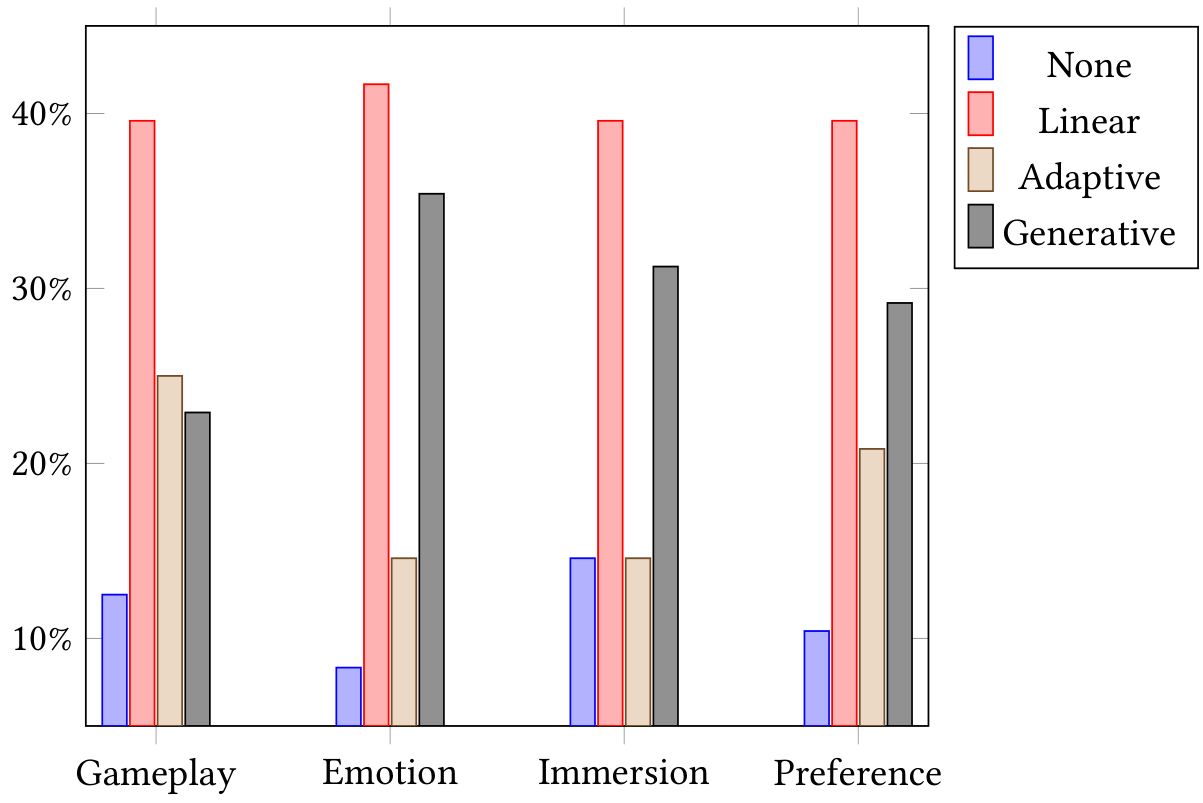
\includegraphics[width=1\linewidth]{images/preglamm_mmm_questionnaire_responses.png}
    \caption{Distribution of questionnaire responses \cite{plut2022preglam}}
    \label{fig:preglamm_mmm_questionnaire_responses}
\end{figure}
In addition, Plut et al. suggest that linear and adaptive music may feel repetitive after a certain time \cite{plut2022preglam}. This could lead to generative music being preferred more likely after several repetitions of game, as it offers new musical content.

\subsection{Limitations}
When comparing the results of the studies, it is important to note that while the generative score in the third study creates unique music customized to the gameplay, the system does not support real-time generation \cite{plut2022preglam}. Although Plut et al. believe, that the musical variety is not noticeably influenced for the participants of the study \cite{plut2022preglam}, the results could still have been affected by this factor. 

Considering the disadvantages and technical challenges, generative music systems like MMM \cite{ens2020mmm} can be highly resource-intensive and computationally demanding \cite{plut2022preglam}. Plut et al. had to pre-generate music for their evaluation because the model was too slow to generate music in real-time \cite{plut2022preglam}.

As previously mentioned, the consistency, predictability, and reliability of adaptive and generative music systems are often problematic when compared to the quality of hand-composed music. While adaptive music can generally be better controlled, it is still not entirely predictable due to the system's deep integration into the game and its dependency on numerous variables.

Another challenge in adaptive music is ensuring that individual musical sections meet the necessary musical requirements. Theoretically, these sections could be composed independently of one another. However, in order to allow for as many possible combinations of the sections, they are often created with similar characteristics, such as tempo or key \cite{plut2020generative}. This approach is showcased in the video game "Red Dead Redemption" \cite{reddeadredemption2010}, where different musical sections are composed in the same key and tempo to support smooth transitions \cite{plut2020generative}.
While this strategy ensures seamless transitions, it can also limit musical variety and diversity. If the sections are composed with distinct musical characteristics, it may increase the complexity of combining them and require more implementation effort.


\subsection{Impact}
When implemented effectively, both adaptive and generative music can significantly enhance how the players connect with and enjoy video games. This result from the scientific work presented could engage game developers to implement adaptive and generative systems in video games. 
Nevertheless, it can be said that generative scientific models, such as MMM \cite{ens2020mmm}, are not yet practically usable in real-time applications due to their high resource demands. This, on the other hand, could encourage other researchers to enhance existing generative music models and algorithms or to develop new, improved ones.